\subsection{External Interface Requirements}
\subsection{Performance Requirements}
\subsection{Design Constraints}
\begin{enumerate}
	\item Query caching
	\newline
	In order to avoid traffic requests to the database and to speed up database , query caching is crucial. AdoDB provides powerful caching system which can implemented in the navUP system and help improve speed regarding interaction between front end and database.
\end{enumerate}
\subsection{Software System Attributes}
\begin{enumerate}
	\item Security
	\newline
	The navUP system will need to adhere to the highest security standards because of the personal information of users that will be stored. In order to achieve security , The navUP system needs to store users’ information and the passwords should be stored in the database as encrypted to remain hidden from the unauthorised users  .
	\item Performance
	\newline
	The system should ensure that basic operations like user registration , user login should be of maximum speed. 
	\item Availability
	\newline
	The navUP system will need to be connected to the internet to ensure that the system can communicate with  the database.
	\item Reliability
	\newline
	The navUP system will need to work roburstly without any failures including failure to retrieve information from the database.
\end{enumerate}
\subsection{UML diagrams}
\subsubsection{Class diagram}
\begin{figure}[H]
	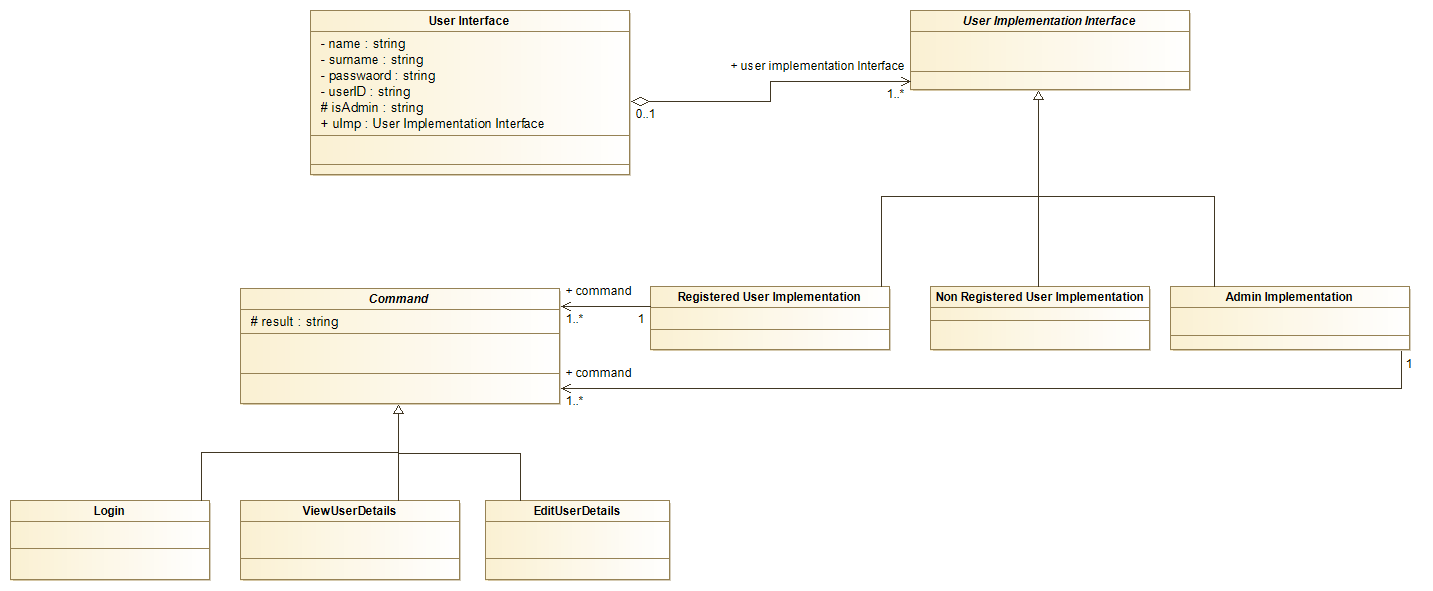
\includegraphics[width=12cm,height=26cm,keepaspectratio]{Users/Pictures/User_Class_Diagram.png}
	\caption{Class diagram for user management module}\label{visina8}
\end{figure}
\subsubsection{Activity diagram}
\begin{figure}[H]
	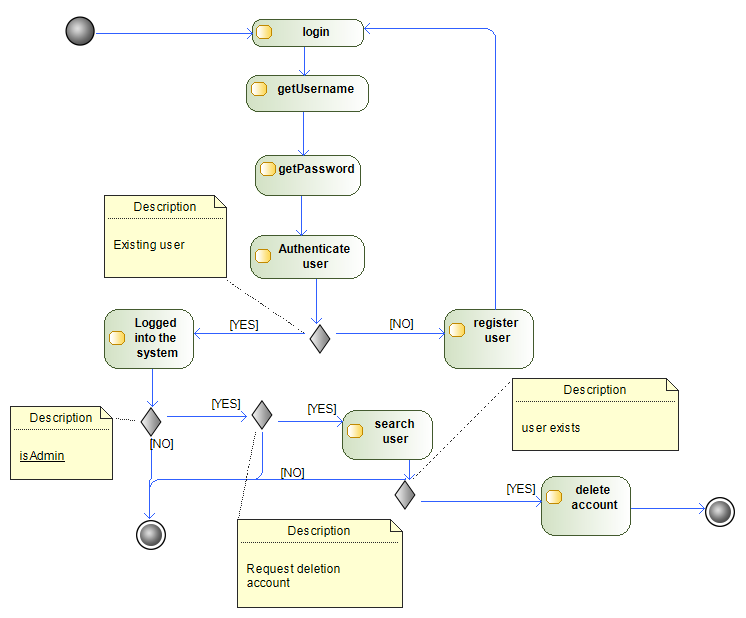
\includegraphics[width=12cm,height=26cm,keepaspectratio]{Users/Pictures/user_Activity_diagram.png}
	\caption{Activity diagram for user management module}\label{visina8}
\end{figure}
\subsubsection{State diagram}
\begin{figure}[H]
	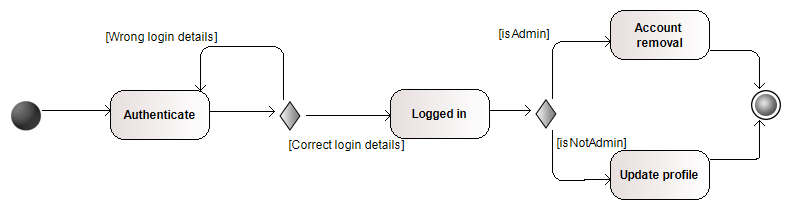
\includegraphics[width=12cm,height=26cm,keepaspectratio]{Users/Pictures/User_State_Diagram.png}
	\caption{State diagram for user management module}\label{visina8}
\end{figure}
\subsubsection{Use Case diagram}
\begin{figure}[H]
	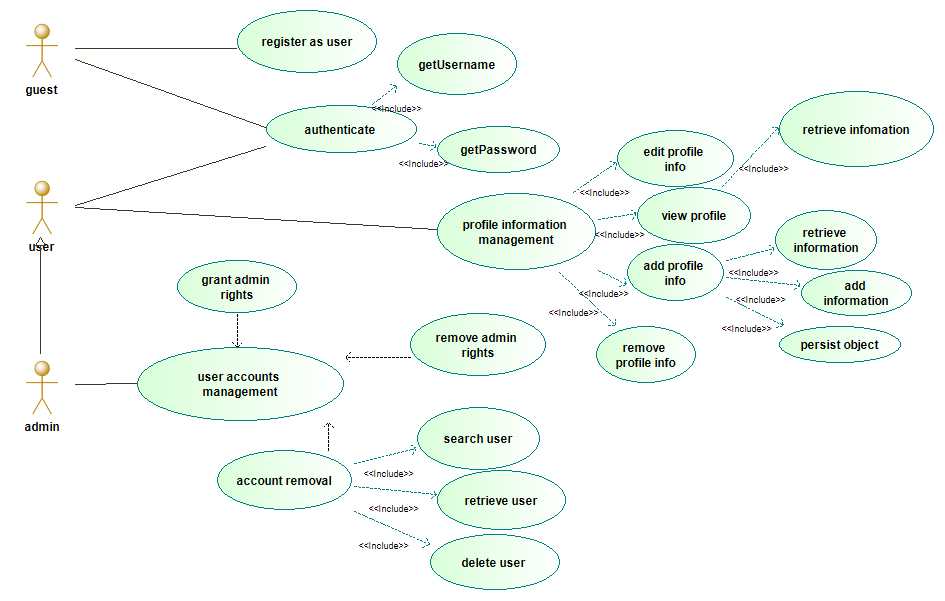
\includegraphics[width=12cm,height=26cm,keepaspectratio]{Users/Pictures/user_use_case_diagram.png}
	\caption{Use case diagram for user management module}\label{visina8}
\end{figure}
